\documentclass[11pt]{article}
\usepackage{graphicx}
\usepackage{booktabs}
\usepackage{multirow}
\usepackage{natbib}

\title{A Multi-file Demo Manuscript}
\author{Demo Author}
\date{}

\begin{document}
\maketitle

\section{Introduction}
Multi-file projects split chapters into \texttt{sections/}. Cross-file references must still resolve:
Section~\ref{sec:method} describes the pipeline, and the key result is in Figure~\ref{fig:res}.

% 下面这行是注释，里面提到 \toprule 与 \cite{ghost2099}，静态检查不应把它算违规

\section{Methods}
\label{sec:method}
The pipeline runs static checks first and then compiles to convergence.
We build on prior work \citep{sheng2021} and a second reference \citet{wang2020}.

\begin{tabular}{lcr}
\toprule
step & cost & note \\
inspect & 1 & static \\
compile & 3 & rounds \\
\bottomrule
\end{tabular}


\section{Results}
The method is compared with earlier work \cite{sheng2021,wang2020}.
Table~\ref{tab:main} lists the settings and Figure~\ref{fig:res} shows the trend.

\begin{table}[h]
\centering
\begin{tabular}{lcr}
\toprule
setting & value & unit \\
temperature & 25 & C \\
pressure & 12 & MPa \\
\bottomrule
\end{tabular}
\caption{Main settings.}
\label{tab:main}
\end{table}

\begin{figure}[h]
\centering
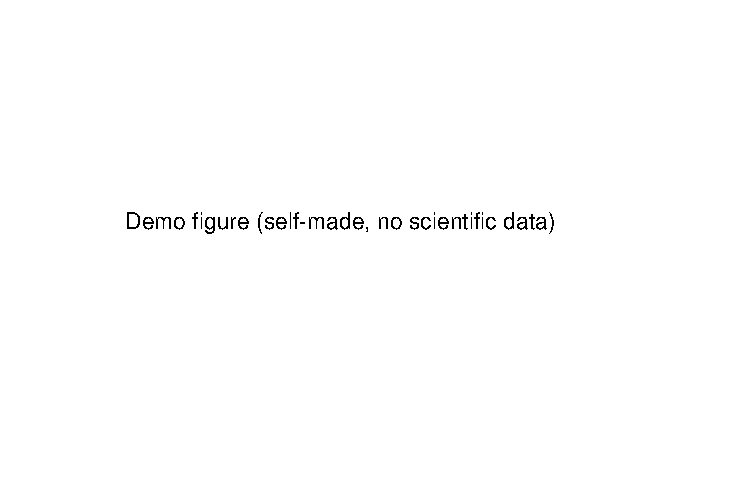
\includegraphics[width=0.8\linewidth]{figs/result.pdf}
\caption{Demo figure from a subdirectory.}
\label{fig:res}
\end{figure}

\section{Conclusions}
The multi-file manuscript compiles with cross-references and citations resolved.

\bibliographystyle{plain}
\bibliography{refs}

\end{document}
